\chapter{Pose Estimation Development}
\label{chapter4}

\section{RGB-to-RGBD}

Various approaches were discussed during the background and research chapter to solve the human-robot distance problem. Two of these methods base their working solution on the RGB-D sensor, which luckily comes integrated on TIAGo, while the third and last approach is more of a generic one as it only requires RGB data for it to work.

Therefore, from a point of view of user reachability it would have made more sense to use the triangulation process as most robotics systems nowadays are equipped with cameras for their perception. Moreover, given the availability of fully functional triangulation routines in OpenCV would have made the implementation of the triangulated solution easy as well. However, such approach would require having a minimum of two cameras mounted on the robot to find corresponding points and apply the epipolar geometry equations presented in Chapter2, which wasn't the case, and although the issue could have been patched by taking different frames of the same view from different position by moving the robot slightly in the environment it would have made the whole process less smooth as continuous movement would have been required to keep updating the distances.

Another viable approach was to use the Point-Cloud-Library (PCL) library and its implementation of a Histogram of Oriented Gradients based detection module able to detect people in RGB-D data. However, although the detection was claimed to be possible in real-time using standard CPU time, only people standing or walking and generally in up-right positions were possible to detect, which did not make sense, especially when a more reliable and sophisticated method such as the RGB person recognition was available.

Hence the decision to use the integrated RGB-D camera and the already available depth-map with per-pixel distance. This, overall, was a better choice to make, as it reduced the implementation time given that no added routine of logic was needed and reducing at the same time the computational costs given that just mere msg conversions and indexing were actually needed to obtain a rather accurate distance estimation.
\clearpage

\section{Development Phases}

The overall pose retrieval logic was split in two phases, a depth one and a pose one. The depth phase uses the RGB detection results and finds the corresponding centre point in the synchronised depth-image, thereby obtaining the resulting human-robot distance per detection. The pose phase uses the retrieved distance to compute the real world pose of the person, where by real world pose in this case is meant the map frame.

\section{Depth Phase}

As previously mentioned the depth phase part of the \textbf{getPoses} function in the \textbf{pose\_finding.py} script which implements the module as a class, makes use of the detection results whose integration with the pose estimation module is presented in details in Chapter6, but from an outline point of view for each detection available the centre point of the bounding box, in terms of x and y given the 2D space, are accessed and the corresponding pixel is indexed in the depth image, itself converted into an appropriate OpenCV format for the processing. Moreover, the RGB-D measurements are subject to noise and therefore an average distance is computed over the neighbouring pixels of the centre coordinate so as to allow a more robust distance estimation. Below is an outline of the depth phase steps:

\begin{enumerate}
  \item Convert depth-image into 32FC1 encoding
  \item Process the ROI (Region of Interest) and compute the average distance
  \item Publish distance message
\end{enumerate}

\subsection{32FC1 conversion}

The first step towards obtaining the required ROI for the distance computation is the conversion of the depth-image into a 32FC1 encoded OpenCV image, where this means that each pixel value is stored as one channel floating point with single precision.

The conversion process is similar if not identical to what was done with RGB msg for the detection module, with the only difference, of course, in the encoding. The result obtained from the conversion consists in a \textbf{float32} numpy array where each pixel is 1:1 mapped to every raw RGB pixel storing the corresponding distance value in metres.

\begin{lstlisting}
    	  # Convert depth-image into a float32 array of metre values
        cv_depth_image = CvBridge().imgmsg_to_cv2(depth_raw_image, '32FC1')
\end{lstlisting}

\subsection{ROI processing \& Depth computation}

The ROI extraction process makes use of three variables: d, x, and y. The variable d is the size of the neighbours around the centre point or how far shall the ROI look into to compute the average distance, while the x and the y are the detection's bounding box centre point.

RGB-D values can be noisy, in fact, the sensor has a minimum and maximum range where the values aren't always assured to be valid, as these in-range values' beams can hit on particular textures or rather complicating objects such as human's ribs, hence the need for a mean distance.

The previously converted depth=image is used to fetch all the values \textbf{d} away from the centre point using Python's slicing feature that enables the retrieval of values within an array, in this case a numpy array, by using simple range indexing. The ROI obtained however, is still not ready to be used, as it might contain invalid values for reasons previously explained which would make the computation fail. Hence numpy's \textbf{np.isnan} functionality is used along with the negation feature \textbf{~} to strip away from the array all invalid values, which in this case occur to be defined as NaN. The result from the stripping process is then used to compute the average distance by using the \textbf{sum} and \textbf{size} routines from numpy's library to get the overall sum of all array's elements and its size.

\begin{lstlisting}
    # Retrieve region of interest
    roi = cv_depth_image[j-d:j+d+1, i-d:i+d+1]
    
    # Filter invalid NaN values
    roi = roi[~np.isnan(roi)]
    
    # Compute average distance
    average_distance = np.sum(roi) / roi.size
\end{lstlisting}

\subsection{Publish distances}

The computed distances for each detection are published over a topic called \textbf{distances} created using the \textbf{Publisher} routine available through the rospy interface, and which publishes custom \textbf{Detections} messages. 

In fact, two custom messages were created for the publishing process, these are the \textbf{Distance.msg}, which holds the distance value in a built-in float64 ROS primitive for each detection along with the latter's ID, defined as an int32 primitive, to have a way to correspond each distance with the correct RGB detection and the \textbf{Distances.msg} that offers an array field of type \textbf{Distance} to hold such objects.

Syntactically the creation of such objects is similar to every other instantiation in Python which sees the name of object class followed by parentheses. To access the relative object's fields the dot operator is used. Moreover, given that the two messages are defined within the package namespace, these have to be imported from it. The message's declaration are shown below:

% \begin{figure}[H]
%     \begin{subfigure}{.5\textwidth}
%       \centering
%       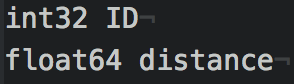
\includegraphics[width=.8\linewidth]{images/chapter4_distance_message.png}
%       \caption{Distance.msg}
%       \label{fig:distance}
%     \end{subfigure}%
    
%     \begin{subfigure}{.5\textwidth}
%       \centering
%       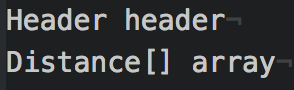
\includegraphics[width=.8\linewidth]{images/chapter4_distances_message.png}
%       \caption{Distances.msg}
%       \label{fig:distances}
%     \end{subfigure}%
% \end{figure}

A distance message is built for every detection and ultimately pushed to the distances collection using a simple \textbf{append} on the array field. Ultimately, the whole collection is published over the topic using the publisher instance described at the beginning. The following is a screenshot of the resulting published message obtained using the \textbf{echo} command on ROS:

TODO: ADD SCREENSHOT OF THE Distance message
\clearpage

\subsection{Ratio offset}

The process of the pose estimation is such that it forms a chain, as the depth module uses the RGB detections, and the depth value itself is used by the pose component for the back-projection and spatial transformations. Therefore, a mistake at an early stage would cause the error to propagate through the chain.

The initial detection stage, that made use of the neural network for the person detection takes as input a 300x300 pixel resolution due to the mechanics of the network. However, the depth-image obtained after the conversion has a resolution of 640x480 pixels, meaning that the assumed 1:1 mapping of the centre location of the bounding box (computed on the 300x300 RGB image) is not correct as the two resolutions differ. This circumstance was not taken into consideration at first and brought some meaningful errors in the distance computation, as the wrong ROI was indexed in the converted depth-image and therefore the wrong distance values were used.

\begin{figure}[H]
	\centering
    \begin{subfigure}{.6\textwidth}
      \centering
      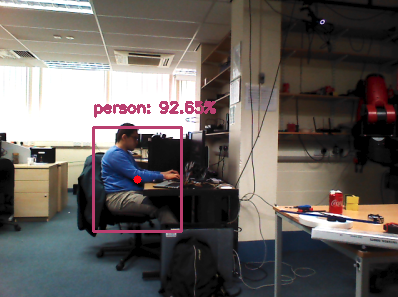
\includegraphics[width=8cm]{images/chapter4_rgb_ratio.png}
      \caption{RGB detection.}
      \label{fig:ratin}
    \end{subfigure}%
    
    \begin{subfigure}{.6\textwidth}
      \centering
      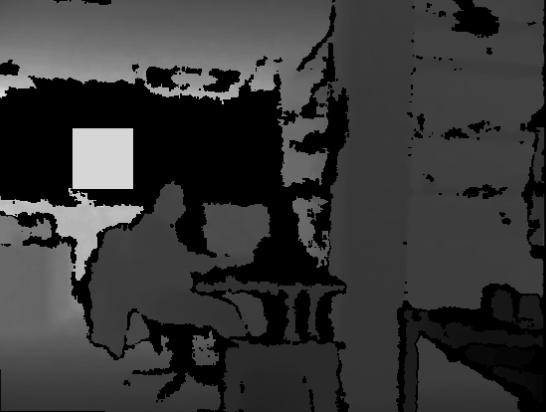
\includegraphics[width=8cm]{images/chapter4_rgbd_no_ratio.png}
      \caption{RGB-D image with ROI.}
      \label{fig:ration}
    \end{subfigure}%
    
    \caption{Ratio offset between the actual centre point and the ROI.}
\end{figure}
\clearpage

The solution to the problem consisted in using ratios, to find the corresponding centre point of the bounding box in the 300x300 image within the 640x480 depth-image. Hence given the x and y coordinates of the centre point and where x represents the width of the image and y the height, the respective coordinates in the depth-image resolution become:

\[x_n = (x/400) * 640 \]
\[y_n = (y/300) * 480 \]

and by converting each detection's centre point prior to the depth module call a correct ROI retrieval is obtained as shown in the figures below:

\begin{figure}[H]
	\centering
    \begin{subfigure}{.5\textwidth}
      \centering
      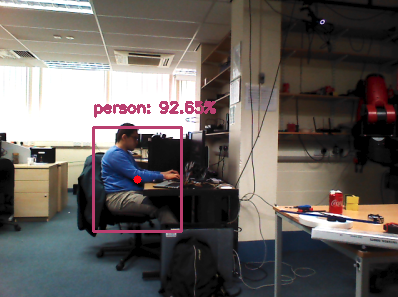
\includegraphics[width=8cm]{images/chapter4_rgb_ratio.png}
      \caption{RGB detection.}
      \label{fig:ratin}
    \end{subfigure}%
    
    \begin{subfigure}{.5\textwidth}
      \centering
      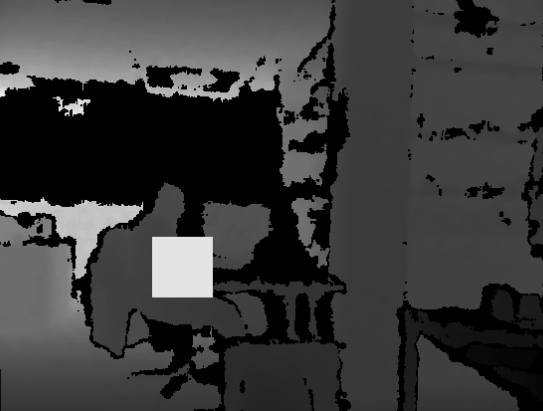
\includegraphics[width=8cm]{images/chapter4_rgbd_ratio.png}
      \caption{RGB-D image with ROI.}
      \label{fig:ration}
    \end{subfigure}%
    
    \caption{Correct point correspondence between the actual centre point and the ROI.}
\end{figure}

\section{Pose phase}

The pose phase where the actual map location of the detection is found has to it three different steps, below outlined:

\begin{enumerate}
  \item Project the bounding box centre point within the RGB optical frame
  \item 3D conversion 
  \item Publish markers and the custom message
\end{enumerate}

\subsection{Pixel Projection}

The pixel back-projection is the inverse process of the original pinhole camera model mapping process, that uses a projection matrix to map 3D world's points to 2D points in the image plane shown below:

\begin{figure}[!htbp]
\begin{center}
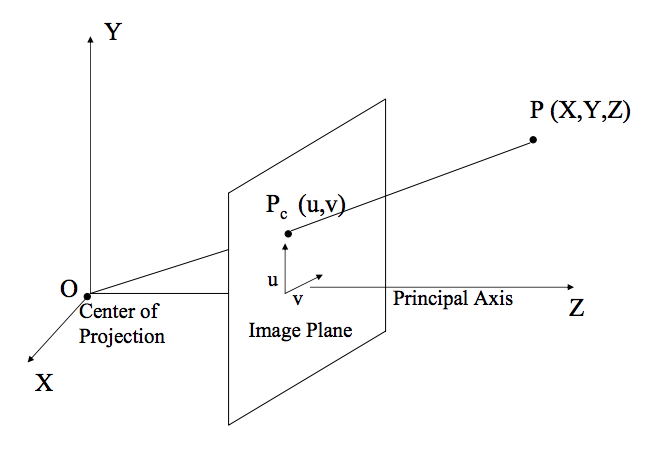
\includegraphics[width=7cm]{images/chapter4_pinhole_model.png}
\end{center}
\caption{Pinhole model (Add reference)}
\label{fig:pinhole}
\end{figure}

The projection matrix used is the union of the intrinsic and extrinsic camera parameters, which are defined via the calibration process. In this occasion, no calibration was required as the RGB was already calibrated by default and the required matrices were made available in TIAGo through ROS.

The \textbf{PinHoleCameraModel} library available in Python was used to obtain the image plane 3D ray. However, before using the class' routines an initial camera info initialisation is needed, hence why a subscription to the \textbf{/xtion/rgb/camera\_info} is made whose callback calls the \textbf{fromCameraInfo} setup routine where the camera's matrices including the distortion and projection one are passed to the instance.

Once the initialisation is complete, the 3D ray can be found by simply calling the \textbf{projectPixelTo3dRay} routine which takes as an argument a tuple containing the coordinates of the RGB pixel to be projected, in this case the centre of the bounding box of the detection, with the first entry being the y coordinate and the second entry the x coordinate. The returned point is then used to find the ultimate 3D point.

\subsection{3D conversion}

All of the required data for the correct 3D pose estimation of the person are now known, the image plane coordinates and the depth, which aggregated together by using a ROS \textbf{Pose} message, gives the 3D vector point with respect to the RGB optical frame. However, the real interest is in knowing the 3D point with respect to the map, as this can then be used to send navigation commands followed by possible interaction features. Therefore, further steps are required.

These steps consist in using spatial transformation to find the rotation matrix which multiplied by the \textbf{PointStamped} transformed 3D point yields the map coordinate of the person. The \textbf{PointStamped} message is merely the same as the \textbf{Pose} message with the addition of a standard ROS header containing a stamp and frame\_id field required for the spatial transformation, and which have respectively been populated with the latest time and the original coordinate frame of the 3D point, in this case \textbf{xtion\_rgb\_optical\_frame}, as follows:

\begin{lstlisting}
	transformHeader = Header()
	transformHeader.stamp = rospy.Time(0)
	transformHeader.frame_id = "xtion_rgb_optical_frame"
\end{lstlisting}

With the transformation made, the \textbf{transformPoint} routine available in the \textbf{tf} package is used to convert the 3D point from one coordinate frame to another. The routine takes two arguments, the first one is the target coordinate frame, the map, while the second one is the point to be converted, the PointStamped instance. The coordinate frame to transform from is contained in the 3D point passed, and is going to be extracted from its header by routine itself, hence why the need for the previous step.

\subsection{Topic Message \& Markers}

Similarly to what was done with the two previous modules, a custom message published over a \textbf{poses} topic was created to let the users subscribe to it and access the computed detections' locations. Hence, a \textbf{Pose} message was declared that holds the single detection pose through a standard ROS Point type, which contains the x, y and z coordinates as float64, as well as the usual ID field necessary to match which pose is to which detection. The Poses message is a collection one that groups together the single instances, and where its declared fields are a header, required by the publisher routine and an array of type Pose. Again, both messages are populated using standard Python field accessing.

Visual markers were used as well to show the detections' pose on RVIZ. To create a marker for each detection, the standard ROS Marker was populated in the \textbf{createMarker} helper function defined in the \textbf{pose\_finding.py} script, where several fields were populated, including colour, scale and marker's coordinates among others. Moreover, for the message to be visualisable in RVIZ, the message had to be specifically published over the \textbf{visualization\_marker\_array} topic as a \textbf{MarkerArray} type, hence the created markers had to be aggregated together. The following is a screen-shot showing how the marker are visualised on RVIZ.

TODO add picture.
\clearpage



